\lysh{26895}{4}
\begin{alist}
\item 
\begin{rlist}
\item Έχουμε $2x + y = 20 \Leftrightarrow y = 20 - 2x \quad (1)$.

Οπότε $xy \overset{(1)}{=} x(20 - 2x) = 20x - 2x^2$. Τελικά η συνάρτηση ως προς $x$ που δίνει το γινόμενο των δύο αριθμών είναι η $f(x) = -2x^2 + 20x$.

\item Από την εκφώνηση έχουμε $x > 0$ και $y > 0$. Όμως $2x + y = 20 \Leftrightarrow y = 20 - 2x$.

Άρα, επειδή $y > 0$, έχουμε $20 - 2x > 0 \Leftrightarrow 2x < 20 \Leftrightarrow x < 10$, οπότε το $x$ ανήκει στο ανοικτό διάστημα $(0,10)$, δηλαδή $D_f = (0,10)$.
\end{rlist}

\item Η $f$ στο πεδίο ορισμού της είναι παραγωγίσιμη, με $f'(x) = -4x + 20$.

Έχουμε $f'(x) > 0 \Leftrightarrow -4x + 20 > 0 \Leftrightarrow x < 5$, επομένως $f$ γνησίως αύξουσα για $x \in (0,5]$. Αντίστοιχα $f'(x) < 0 \Leftrightarrow -4x + 20 < 0 \Leftrightarrow x > 5$, επομένως $f$ γνησίως φθίνουσα για $x \in [5,10)$.

\item Από το β) ερώτημα συμπληρώνουμε τον παρακάτω πίνακα μεταβολών

\begin{center}
\begin{tikzpicture}
\tikzset{arrow style/.style={maincolor,>->,>=latex'}}
\tikzset{t style/.style = {style = dashed}}
\tikzset{z style/.style = {fill=white,inner sep=.2mm}}
\tkzTabInit[color,lgt=2,espcl=2.4,colorC = maincolor!50,colorL = maincolor!30,colorV = maincolor!50]%
{$x$ / .8,$f'$ /.8,$f$/1.2}%
{$0$,$5$,$10$}%
\tkzTabLine{,+,z,-,}
\tkzTabVar{-/ , +/ \text{O.M.} , -/ }
\end{tikzpicture}
\end{center}

Οπότε η $f$ παρουσιάζει μέγιστο για $x=5$, $f(5) = -2 \cdot 5^2 + 20 \cdot 5 = 50$.
\end{alist}
\vspace{6mm}
\noindent\rule{\textwidth}{0.4pt}
\vspace{6mm}

